% measuring-the-moat.tex --- version 2.0 (2026-07-26).
%
% Version 1.1 (2026-07-23) is frozen as
% note_draft_v1.tex and is not edited by this file.  What changed:
%
%   - the upper bound is now a single flat theorem (Thm 2.6) covering every
%     n >= 24; the pure-ring, cycle-power and keystone-transplant bounds of
%     v1.1 are all subsumed by it and are kept only as provenance
%   - Prop 4.1 of v1.1 (E(17) >= 3, computer-assisted, CP-SAT 357 s) is
%     replaced by Prop 3.1, an elementary statement determining E on the whole
%     family n = 2k+1, delta+ >= k.  The solver runs are demoted to a record
%     of where the direct model reaches
%   - a class-limited partial lower bound is added (Thm 4.1, Appendix B)
%   - E_delta and E_delta^sc are now defined separately; v1.1 defined only the
%     strongly connected one while the repository README defined the other
%   - the word "floor" is reserved for E itself throughout
%   - Section 6 (structure of witnesses) withdraws a reading of v1.1: the two
%     analysed witnesses are now known not to be optimal
%
% Table in Section 5.1 is machine-generated by make_table.py (do not hand-edit).
\documentclass[11pt]{amsart}
\usepackage{amsmath,amssymb}
\usepackage[hidelinks]{hyperref}
\usepackage{booktabs}
\usepackage{tikz}

\newtheorem{theorem}{Theorem}[section]
\newtheorem{lemma}[theorem]{Lemma}
\newtheorem{conjecture}[theorem]{Conjecture}
\newtheorem{proposition}[theorem]{Proposition}
\theoremstyle{remark}
\newtheorem{remark}[theorem]{Remark}

\newcommand{\exc}{\operatorname{exc}}
\newcommand{\Esc}{E^{\mathrm{sc}}}

\title[Measuring the moat]{Measuring the moat: excess bounds near
Seymour's second neighbourhood conjecture}

\author{Daiki Tahara}
\address{Independent researcher, Osaka, Japan}
\thanks{Version 2.0 --- 2026-07-26. Supersedes version 1.1 (2026-07-23),
which remains archived; no claim of that version became false.}

\begin{document}

\begin{abstract}
Seymour's second neighbourhood conjecture (SSNC) asserts that every oriented
graph has a vertex whose second out-neighbourhood is at least as large as its
first. For an oriented graph $G$ define
$\exc(G) = \sum_v \max(0,\, d_2(v) - d_1(v) + 1)$; then $\exc(G) = 0$ iff $G$
is a counterexample. Let $E_{\ge d}(n)$ be the minimum excess over $n$-vertex
oriented graphs of minimum out-degree at least $\delta$, and $\Esc_{\ge d}(n)$
the same minimum over the strongly connected ones. We prove
$E_{\ge 8}(n) \le \Esc_{\ge 8}(n) \le 3 + [3 \nmid n]$ for every
$n \ge 24$, by exhibiting one explicit family; this subsumes every upper bound
of the previous version. At the opposite extreme we determine $E$ exactly on a
degenerate family: $E_{\ge k}(2k+1) = 2k+1$ for all $k \ge 1$, by an
elementary argument that replaces a solver computation. Inside one explicitly
defined class of capped-tournament blow-ups we prove a partial lower bound,
$\exc \ge 3$ with equality forcing $3 \mid n$; we emphasise that this says
nothing outside that class. No lower bound is known at any $n \ge 18$. We also
record, as a methodological result, that search attainment overstated the
best available upper bound in every discrepancy, and that in each case an
explicit construction, not a further search, settled it.
\end{abstract}

\maketitle

\section{Introduction}

Seymour's second neighbourhood conjecture \cite{DeanLatka1995} states:

\begin{conjecture}[SSNC]
Every oriented graph (digraph without 2-cycles) contains a vertex $v$ with
$|N_2^+(v)| \ge |N_1^+(v)|$.
\end{conjecture}

The conjecture is proved for tournaments \cite{Fisher1996,HavetThomasse2000}
and in many special classes; every oriented graph has a vertex with
$|N_2^+(v)| \ge \gamma\,|N_1^+(v)|$ for $\gamma = 0.715538\ldots$
\cite{HuangPeng2024}, improving \cite{ChenShenYuster2003}. A counterexample
must have minimum out-degree $\delta^+ \ge 8$: out-degree $\le 6$ was
eliminated by \cite{KanekoLocke2001} and $\delta^+ = 7$ by
\cite{SadhukhanSandeepSen2026} via a signature-compression argument checked by
CP-SAT.

Recent work studies the \emph{equality boundary} of the conjecture.
\cite{Halkiewicz2026} calls a strongly connected oriented graph \textbf{Pisa}
if $\max_v (|N_2^+(v)| - |N_1^+(v)|) = 0$; \cite{GuoKangZwaneveld2026} study
\textbf{Seymour-tight} orientations, in which \emph{every} vertex meets the
bound, and develop a product calculus for them. In the tight case the set of
boundary vertices is everything; in a generic Pisa graph it can be much
smaller. This note measures how small.

\subsection*{Definitions}
For an oriented graph $G$ write $d_1(v) = |N_1^+(v)|$ and
$d_2(v) = |N_2^+(v)|$, where $N_2^+(v) = \{x : \operatorname{dist}^+(v, x) =
2\}$; so $N_1^+(v)$, $N_2^+(v)$ and $\{v\}$ are pairwise disjoint. Call
$m(v) = d_2(v) - d_1(v)$ the \emph{margin} of $v$, call $v$ \textbf{tight} if
$m(v) = 0$ and \textbf{satisfied} if $m(v) \ge 0$. Define
\[
\exc(G) \;=\; \sum_{v \in V(G)} \max\bigl(0,\; m(v) + 1\bigr).
\]
Then $\exc(G) = 0$ iff $G$ is a counterexample to SSNC, and for a Pisa graph
the excess equals the number of tight vertices. Adding a universal sink
produces $\exc = 1$ trivially \cite[\S1]{GuoKangZwaneveld2026}, so the
interesting quantity carries the degree bound that counterexamples must
satisfy. \emph{Two} minima are used here and they must not be conflated:
\begin{align*}
E_{\ge d}(n) &= \min\{\exc(G) : |V(G)| = n,\ G \text{ oriented},\
   \delta^+(G) \ge \delta\},\\
\Esc_{\ge d}(n) &= \text{the same minimum over the strongly connected such } G.
\end{align*}
Since the second minimises over a subclass, $E_{\ge d}(n) \le \Esc_{\ge d}(n)$.
Version 1.1 of this note defined only $\Esc$, writing it $E$, while the
accompanying repository defined only $E$; the two were used interchangeably.
They are separated here, and every statement below says which one it bounds.
The reasons are uniform: an upper bound witnessed by a strongly connected
graph bounds both, and an infeasibility argument run without a connectivity
constraint rules out the larger class and hence the subclass as well. The
restriction to strong connectivity is motivated by the minimal-counterexample
reduction --- a closed out-section of a counterexample is a smaller
counterexample, cf.\ \cite{EspunyDiazGiraoGranetKronenberg2024}.

$E_{\ge 8}(n) = 0$ for some $n$ iff SSNC is false. If SSNC holds then
$E_{\ge 8}(n) \ge 1$ for all $n$, and any stronger uniform lower bound
is a strengthening of the conjecture.

\subsection*{Terminology: floor, bound, attainment}
Version 1.1 and the repository README used the word ``floor'' for values
reached by search. They are not floors, and the improvements reported here are
what made that visible. Three words are kept apart throughout:
\emph{floor} means $E_{\ge d}(n)$ itself, the exact minimum --- which we do not
know at a single $n \ge 18$; \emph{bound} means a proved inequality; and
\emph{attainment} means the best value some search actually reached, which is
evidence for an upper bound and never for a lower one. Section~\ref{sec:notfloor}
is the record of what happens when the three are mixed.

\subsection*{Contributions}
\begin{enumerate}
\item \textbf{A flat upper bound} (\S\ref{sec:constructions}): one explicit
  family gives $\Esc_{\ge 8}(n) \le 3 + [3 \nmid n]$ for every
  $n \ge 24$ (Theorem~\ref{thm:flat}). It subsumes the pure-ring,
  cycle-power and keystone-transplant bounds of version 1.1, which are
  retained as provenance in \S\ref{sec:legacy}.
\item \textbf{An exact value on a degenerate family} (\S\ref{sec:lower}):
  $E_{\ge k}(2k+1) = \Esc_{\ge k}(2k+1) = 2k+1$ for every
  $k \ge 1$ (Proposition~\ref{prop:odd}), by six lines of argument. The
  $k = 8$ case supersedes the computer-assisted $E(17) \ge 3$ of version 1.1.
\item \textbf{A class-limited partial lower bound} (\S\ref{sec:class},
  Appendix~\ref{app:class}): inside one explicitly defined family of
  capped-tournament blow-ups, $\exc \ge 3$, with equality forcing
  $3 \mid n$. This is \emph{not} a lower bound on $E_{\ge 8}$.
\item \textbf{Measurements and a measurement-theoretic caveat}
  (\S\ref{sec:measurements}): search attainment was wrong in both
  directions, and construction alone adjudicated each time.
\item \textbf{Open problems} (\S\ref{sec:open}), foremost: is
  $3 + [3 \nmid n]$ exact? Nothing is known on the lower side at any
  $n \ge 18$.
\end{enumerate}

\subsection*{Verification protocol}
Every witness is stored in the accompanying repository as an adjacency list
with a SHA-1 fingerprint, and every numerical claim is checked by
implementations written independently of one another: a numpy pipeline used by
the search, a pure-Python verifier, and a standard-library-only verifier
written from the definitions without access to the other two. A
\texttt{make verify-*} target reproduces each claim, and every claim in the
repository's table has one. The solver logs are \emph{not} uniform in
provenance; \S\ref{sec:provenance} states exactly which fields each records.

\section{The flat upper bound}\label{sec:constructions}

\subsection{The out-set inclusion lemma}

All constructions here are perturbed blow-ups of directed cycles. The
mechanism that keeps perturbations from leaking is the following.

\begin{lemma}[out-set inclusion]\label{lem:outset}
Let $G$ be an oriented graph and let $v \ne p$ be non-adjacent vertices with
$N_1^+(p) \subseteq N_1^+(v)$. Let $G' = G + (v \to p)$. Then $G'$ is
oriented, and:
\begin{enumerate}
\item[(i)] if $p \in N_2^+(G, v)$, then $m_{G'}(v) = m_G(v) - 2$;
\item[(ii)] if $p \notin N_1^+(G,v) \cup N_2^+(G, v)$, then
  $m_{G'}(v) = m_G(v) - 1$;
\item[(iii)] for $x \ne v$, margins change only by the possible appearance of
  $p$ in $N_2^+(x)$ through the new path $x \to v \to p$: precisely,
  $m_{G'}(x) = m_G(x) + 1$ exactly when $v \in N_1^+(x)$ and
  $p \notin N_1^+(x) \cup \{x\} \cup N_2^+(G, x)$; all other margins are
  unchanged. In particular, if every in-neighbour $x$ of $v$ satisfies
  $p \in N_1^+(x)$, then no margin other than $m(v)$ changes.
\end{enumerate}
\end{lemma}

\begin{proof}
$G'$ is oriented since $p \to v$ is absent by non-adjacency. For $v$:
$d_1(v)$ increases by exactly one. Candidate new second neighbours of $v$ are
the out-neighbours of the new first neighbour $p$, i.e.\
$N_1^+(p) \setminus (N_1^+(G',v) \cup \{v\}) = \emptyset$ by hypothesis; and
no old second neighbour $u \ne p$ is lost, since arcs are only added and
$u \notin N_1^+(G', v)$. The only possible change to $N_2^+(v)$ is the removal
of $p$ itself, which occurs precisely in case (i); this gives (i) and (ii).
For $x \notin \{v, p\}$: $d_1(x)$ is unchanged, and the only new directed
paths of length two are of the form $x \to v \to p$, which affect membership
of $p$ alone; the stated condition characterises when $p$ actually enters
$N_2^+(x)$. For $x = p$: no new path leaves $p$, and no new path of length two
into $N_2^+(p)$ is created, since such a path would require an arc into $v$ to
be new.
\end{proof}

In words: \emph{if the target's out-set is already inside the shooter's first
neighbourhood, the shot costs the shooter one unit of margin and is invisible
to bystanders who see both.} The same arithmetic underlies the in-star trick
in the generalized lexicographic products of \cite{GuoKangZwaneveld2026}.

\subsection{The family $G_n$}\label{sec:family}

Fix $n \ge 24$ and write $m = \lfloor n/3 \rfloor$, $r = n \bmod 3$. Partition
$V$ into three layers $L_0, L_1, L_2$ of sizes
\[
s_a \;=\; m + [\,a < r\,] \qquad (a = 0,1,2),
\]
so $s_0 + s_1 + s_2 = n$. Layers are consecutive blocks: with
$\mathrm{st}_a = s_0 + \cdots + s_{a-1}$, the $j$-th vertex of $L_a$ is
$u_{a,j} = \mathrm{st}_a + j$. Indices of layers are mod $3$. Put
\[
\Delta_a \;=\; s_{a+2} - s_{a+1}, \qquad
c_a \;=\; \max(0,\, \Delta_a + 1).
\]
The arcs of $G_n$ are exactly
\begin{itemize}
\item[(R)] $u_{a,j} \to w$ for every $w \in L_{a+1}$ (complete, forward);
\item[(T)] $u_{a,j} \to u_{a,l}$ for every $l < \min(j, c_a)$ (an intra-layer
  transitive tournament, truncated at the cap $c_a$).
\end{itemize}

\begin{figure}[h]
\centering
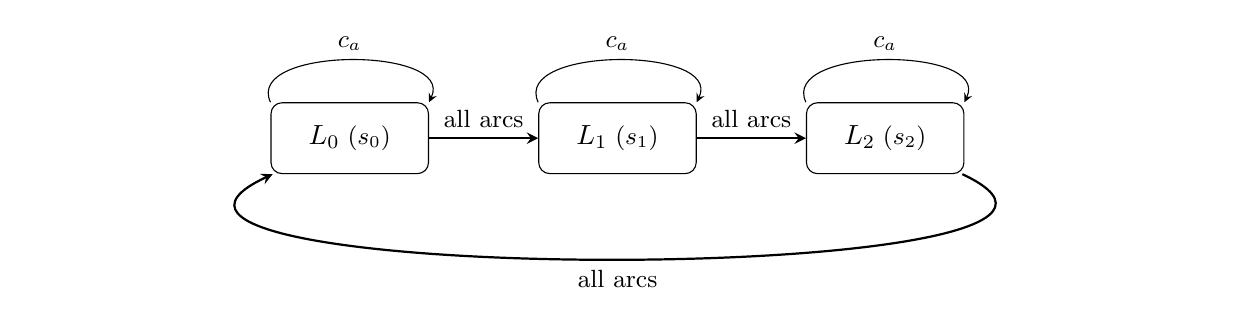
\begin{tikzpicture}[>=stealth, node distance=34mm]
  \node[draw, rounded corners, minimum width=20mm, minimum height=9mm] (L0)
    {$L_0$\;\small$(s_0)$};
  \node[draw, rounded corners, minimum width=20mm, minimum height=9mm,
        right of=L0] (L1) {$L_1$\;\small$(s_1)$};
  \node[draw, rounded corners, minimum width=20mm, minimum height=9mm,
        right of=L1] (L2) {$L_2$\;\small$(s_2)$};
  \draw[->, thick] (L0) -- node[above,font=\small] {all arcs} (L1);
  \draw[->, thick] (L1) -- node[above,font=\small] {all arcs} (L2);
  \draw[->, thick] (L2) to[out=-25,in=-155]
       node[below,font=\small] {all arcs} (L0);
  \foreach \n in {L0,L1,L2}
    \draw[->] (\n.north west) to[out=115,in=65]
       node[above,font=\small] {$c_a$} (\n.north east);
\end{tikzpicture}
\caption{The family $G_n$. Layer sizes are $s_a = \lfloor n/3 \rfloor +
[a < r]$, so they differ by at most one. Between layers, every arc runs
forward; inside a layer, a transitive tournament truncated at the cap $c_a$.
For $v \in L_a$, $N_1^+(v)$ is $L_{a+1}$ together with at most $c_a$
same-layer vertices, while $N_2^+(v) = L_{a+2}$ exactly
(Lemma~\ref{lem:n2}) --- the intra-layer arcs raise $d_1$ without ever
enlarging $N_2^+$.}\label{fig:family}
\end{figure}

\begin{lemma}[well-formedness]\label{lem:wf}
$G_n$ is an oriented graph, is strongly connected, and has
$\delta^+(G_n) = \lfloor n/3 \rfloor$.
\end{lemma}

\begin{proof}
No loops: (T) requires $l < \min(j, c_a) \le j$. No digons: (R) arcs run
$L_a \to L_{a+1}$, and a reverse arc would need $a + 2 \equiv a \pmod 3$;
(T) arcs run strictly downwards in $j$ inside one layer. An (R) arc and a (T)
arc never join the same pair. Out-degrees: $\deg^+(u_{a,j}) = s_{a+1} +
\min(j, c_a) \ge s_{a+1} \ge m$, with equality at $j = 0$ in a layer of
minimum size, so $\delta^+ = m = \lfloor n/3 \rfloor$, which is $\ge 8$
exactly when $n \ge 24$. Strong connectivity: from any $u \in L_a$ every
vertex of $L_{a+1}$ is reached in one (R) step, hence every vertex of
$L_{a+2}$ in two and every vertex of $L_a$ in three.
\end{proof}

\begin{lemma}[second neighbourhood]\label{lem:n2}
$N_2^+(u_{a,j}) = L_{a+2}$, hence $d_2(u_{a,j}) = s_{a+2}$.
\end{lemma}

\begin{proof}
By definition
\[
N_2^+(v) \;=\; \Bigl(\bigcup_{x \in N_1^+(v)} N_1^+(x)\Bigr)
  \setminus \bigl(N_1^+(v) \cup \{v\}\bigr),
\]
so it suffices to compute the union and then delete. Write $p = \min(j, c_a)$,
so $N_1^+(u_{a,j}) = L_{a+1} \cup \{u_{a,0}, \dots, u_{a,p-1}\}$. Every $x \in L_{a+1}$ contributes
$N_1^+(x) = L_{a+2} \cup (\text{some vertices of } L_{a+1})$; $L_{a+1}$ is
non-empty and each such $x$ covers all of $L_{a+2}$, so the union contains
$L_{a+2}$ and nothing outside $L_{a+2} \cup L_{a+1}$. Every $u_{a,l}$ with
$l < p \le c_a$ contributes
$N_1^+(u_{a,l}) = L_{a+1} \cup \{u_{a,0}, \dots, u_{a,l-1}\}$ (using
$l < c_a$), which is contained in $N_1^+(u_{a,j})$ since $l - 1 < j$. So the
two-step reach is $L_{a+2} \cup L_{a+1} \cup (\text{a subset of } N_1^+)$.
Deleting $N_1^+(u_{a,j})$, which contains $L_{a+1}$, and the vertex
$u_{a,j} \in L_a$ leaves exactly $L_{a+2}$, since $L_{a+2}$ is disjoint from
$L_a \cup L_{a+1}$.
\end{proof}

This is the mechanism of Lemma~\ref{lem:outset} in bulk: the intra-layer
targets are chosen so that their out-sets already lie inside the observer's
first neighbourhood, so each (T) arc lowers $d_1 - d_2$ by exactly one without
ever enlarging $N_2^+$.

\begin{lemma}[margins and per-layer excess]\label{lem:layer}
$m(u_{a,j}) = \Delta_a - \min(j, c_a)$. Consequently, writing
$T(x) = (x+1)(x+2)/2$ for $x \ge 0$ and $T(x) = 0$ for $x < 0$,
\[
\sum_{j=0}^{s_a - 1} \max\bigl(0,\, m(u_{a,j}) + 1\bigr) \;=\; T(\Delta_a).
\]
\end{lemma}

\begin{proof}
The first claim is Lemma~\ref{lem:n2} together with
$d_1(u_{a,j}) = s_{a+1} + \min(j, c_a)$. For the sum: when $j \ge c_a$ the
margin is $\Delta_a - c_a \le -1$ and contributes $0$; when $j < c_a$ it is
$\Delta_a - j$, contributing $\max(0, \Delta_a + 1 - j)$, which vanishes once
$j > \Delta_a$. Here $\Delta_a \in \{-1,0,1\}$ by Lemma~\ref{lem:profile}
below, and $s_a \ge 8 > \Delta_a$, so all indices $j = 0, \dots, \Delta_a$
exist and lie below the cap; the sum is
$\sum_{j=0}^{\Delta_a}(\Delta_a + 1 - j) = T(\Delta_a)$ when $\Delta_a \ge 0$,
and $0$ when $\Delta_a < 0$.
\end{proof}

\begin{lemma}[imbalance profile]\label{lem:profile}
From $s_a = m + [a < r]$,
\[
\begin{array}{llll}
r = 0: & (s_0,s_1,s_2) = (m,m,m), &
  (\Delta_0,\Delta_1,\Delta_2) = (0,0,0);\\
r = 1: & (m{+}1,m,m), & (0,+1,-1);\\
r = 2: & (m{+}1,m{+}1,m), & (-1,+1,0).
\end{array}
\]
\end{lemma}

\begin{proof}
Direct substitution into $\Delta_a = s_{a+2} - s_{a+1}$. Note
$\Delta_0 + \Delta_1 + \Delta_2 = 0$ always.
\end{proof}

\begin{theorem}[flat upper bound]\label{thm:flat}
For every $n \ge 24$, the graph $G_n$ is oriented, strongly connected, has
$\delta^+ = \lfloor n/3 \rfloor \ge 8$, and
\[
\exc(G_n) \;=\; 3 + [\,3 \nmid n\,].
\]
Consequently $E_{\ge 8}(n) \le \Esc_{\ge 8}(n)
\le 3 + [3 \nmid n]$ for every $n \ge 24$.
\end{theorem}

\begin{proof}
By Lemmas~\ref{lem:layer} and \ref{lem:profile},
$\exc(G_n) = \sum_a T(\Delta_a)$ with $T(-1) = 0$, $T(0) = 1$, $T(1) = 3$.
For $r = 0$ this is $1+1+1 = 3$; for $r = 1$ it is $1+3+0 = 4$; for $r = 2$ it
is $0+3+1 = 4$. Lemma~\ref{lem:wf} gives the remaining assertions.
\end{proof}

\begin{remark}[the bound does not need $\delta = 8$]\label{rem:delta}
$\delta^+(G_n) = \lfloor n/3 \rfloor$, so the same family gives
$\Esc_{\ge D}(n) \le 3 + [3 \nmid n]$ for every $D \le \lfloor n/3
\rfloor$. The threshold $8$ is not what the construction is responding to.
\end{remark}

\begin{remark}[the Pisa reading is limited to $3 \mid n$]\label{rem:pisa}
When $3 \mid n$ all three $\Delta_a$ vanish and $G_n$ has three tight vertices
and no vertex of positive margin, so it is Pisa and its excess counts tight
vertices. When $3 \nmid n$ some layer has $\Delta_a = +1$ and contributes a
vertex of margin $+1$ (excess $4 = 2 + 1 + 1$); such a $G_n$ is not Pisa.
So the reading of $E_{\ge d}$ as ``the minimum number of margin-$0$ vertices''
is a statement about the subsequence $3 \mid n$, not about $E_{\ge d}$ in
general.
\end{remark}

\subsection{The constructions of version 1.1, and what became of them}
\label{sec:legacy}

Version 1.1 proved $\Esc(mt) \le m$ for $m \ge 3$, $t \ge 8$ (pure rings),
extended it to cycle-power skeletons $\vec{C}_m^{\,k}$, and obtained
$\Esc(n) \le 5$ at $n = 47, 53, 59$ by transplanting a locally rigid cluster
found by search. All three are subsumed numerically by
Theorem~\ref{thm:flat}: at $n = 25, 35, 49$ the cycle-power bound gave $5, 5,
7$ where the theorem gives $4, 4, 4$; at the three primes the transplant gave
$5$ where the theorem gives $4$. The pure ring is the special case $c_a = 1$
of the family above, and $G_n$ is exactly $\vec{C}_3$ blown up with truncated
intra-class tournaments.

The transplant is worth keeping for its mechanism rather than its numbers. It
is built around a \textbf{keystone cluster}: a satisfied vertex $u$ of margin
$+1$ together with \emph{wing} vertices whose out-sets are exact copies of
$N_1^+(u)$ plus the single arc back to $u$ --- out-set inclusion again,
asymmetric and ring-free. We still have no general lemma saying when such a
cluster embeds in a host of prescribed order with controlled excess
(Problem~\ref{prob:transplant}).

\section{An exact value, and the state of the lower bound}\label{sec:lower}

\subsection{A degenerate family where $E$ is determined}

\begin{proposition}\label{prop:odd}
Let $k \ge 1$ and $n = 2k+1$. Every oriented graph $G$ on $n$ vertices with
$\delta^+(G) \ge k$ satisfies $\exc(G) = n$. Hence
$E_{\ge k}(2k+1) = \Esc_{\ge k}(2k+1) = 2k+1$; in particular
$E_{\ge 8}(17) = 17$.
\end{proposition}

\begin{proof}
The arc count of an oriented graph on $n$ vertices is at most $\binom{n}{2}$,
and $\delta^+ \ge k$ forces it to be at least $nk = \binom{2k+1}{2}$. So
equality holds throughout: every pair is adjacent and every out-degree is
exactly $k$, i.e.\ $G$ is a regular tournament.

Fix $v$ and let $w \in N^-(v)$. Suppose $w \notin N_2^+(v)$. For any
$y \in N_1^+(v)$ we have $v \to y$; if $y \to w$ then $v \to y \to w$ is a
path of length two and, since $w \notin N_1^+(v) \cup \{v\}$, this would put
$w \in N_2^+(v)$. As $G$ is a tournament, $w \to y$ instead. Hence
$N_1^+(v) \subseteq N_1^+(w)$; and $w \to v$ gives $v \in N_1^+(w)$ while
$v \notin N_1^+(v)$, so $N_1^+(v) \cup \{v\} \subseteq N_1^+(w)$ and
$|N_1^+(w)| \ge k+1 > k$, contradicting regularity. Therefore
$N^-(v) \subseteq N_2^+(v)$ and $d_2(v) \ge k$. Conversely
$N_2^+(v) \subseteq V \setminus (N_1^+(v) \cup \{v\})$ gives
$d_2(v) \le n - 1 - k = k$. So $m(v) = 0$ at every vertex and $\exc(G) = n$.
Finally $N_2^+(v) = N^-(v)$ puts every vertex within distance two of every
other, so all these graphs are strongly connected and the two minima agree.
\end{proof}

Proposition~\ref{prop:odd} is not new: it is the classical fact that a vertex
of maximum score in a tournament reaches every other vertex within two steps,
applied to a regular tournament where every vertex qualifies; the special case
we need is \cite[Lem.~2.2]{GuoKangZwaneveld2026}. We state it because of what
it replaces. Version 1.1 proved $E_{\ge 8}(17) \ge 3$ from a CP-SAT
infeasibility run of $357$ s, and a later run of $3\,083$ s at a higher cap
pushed the same statement to $\ge 5$. Both are true, and both are strictly
weaker than the six lines above. We record this rather than quietly dropping
it: the computations were sound, and the conclusion they reached was simply
not the strongest available.

\begin{remark}[why $n = 2k+1$ says nothing about anything else]
The hypothesis is doing all the work, and dropping it by one collapses the
value rather than lowering it slightly. At $n = 5$, $k = 2$ the oriented graph
with out-sets $\{3,4\}, \{3,4\}, \{3\}, \{4\}, \{2\}$ is digon-free with
$\delta^+ = 1$ and excess $3$, not $5$. So $E_{\ge 8}(17) = 17$ is an
isolated rigid point: the degree bound pins the class down to a single excess
value, and at $n = 18$ non-tournaments of low excess are immediately
admissible. The large value is \emph{not} evidence for a lower bound anywhere
else.
\end{remark}

\subsection{What is known on the lower side}

Nothing, at any $n \ge 18$. Specifically: for $18 \le n \le 23$ there is no
construction, no lower bound, and no working search instrument (the density
forced by $\delta^+ \ge 8$ leaves almost no legal local moves). For
$n \ge 24$, $3 + [3\nmid n]$ is an upper bound only, and whether it is exact
is open. Any bound of the form $E_{\ge 8}(n) \ge 2$ for all $n$ is
already a strengthening of SSNC restricted to this class; the case
$c = 2$ is the restriction to $\delta^+ \ge 8$ of a conjecture of Dara,
Francis, Jacob and Narayanan \cite{DaraFrancisJacobNarayanan2022} that every
sink-free oriented graph contains at least two Seymour vertices.

\subsection{Where the direct solver model reaches}\label{sec:reach}

The CP-SAT model $M_{n,c}$ of Appendix~\ref{app:model} decides
``$\exc \le c$'' at $n = 17$ for $c = 2, 3, 4$ ($357.0$ s, $1\,356.4$ s,
$3\,083.0$ s, all INFEASIBLE) and returns UNKNOWN at $n = 19$ and $n = 20$
for $c = 3$ within $1\,800$ s each, and at $18 \le n \le 22$ for $c = 2$
within $3\,600$ s each. The tournament-restricted variant of
``$\exc \le 2$'' returned twelve consecutive UNKNOWNs at one hour each over
$17 \le n \le 28$. After Proposition~\ref{prop:odd} the $n = 17$ rows are of
interest only as a measurement of the model: they consumed up to an hour to
establish something a paragraph settles, which is the honest calibration of
how far this approach reaches. It does not reach the orders where the
question is live.

\subsection{Provenance of the solver logs}\label{sec:provenance}

The logs are not uniform, and a reader comparing claims should know which tier
each rests on. Counted field by field over every row:

\begin{center}\small
\begin{tabular}{lrrrr}
log & rows & model hash & solver version & workers \\ \hline
\texttt{gkz82\_results.jsonl} & 25 & 0 & 0 & 0 \\
\texttt{excess2\_results.jsonl} & 8 & 1 & 1 & 0 \\
\texttt{excess3\_probe\_results.jsonl} & 4 & 4 & 4 & 4 \\
\end{tabular}
\end{center}

\noindent The GKZ scan records conjecture, $k$, $n$, two model flags, status
and wall time --- seven fields, except for the rows at $n = 7, 8, 9$, which
predate one of the flags and carry six. The $\exc \le 2$ log carries four
fields on seven of its eight rows and seven on the remaining one, which alone
has a model hash and solver version. The reachability probe carries thirteen
fields on every row, including model hash, solver version and worker count;
none of the three logs records a solver seed. All models are in the repository
and can be re-run; only the third log pins down the binary that produced it.

Two instances of a status changing on re-run are kept in the logs, and they
are not the same phenomenon. In the GKZ scan, $n = 29$ was UNKNOWN at
$14\,400$ s and INFEASIBLE at $29\,506$ s: a budget was exhausted and roughly
twice the budget decided it. In the $\exc \le 2$ log, $n = 17$ was UNKNOWN at
$900$ s and then INFEASIBLE at $218.9$ s --- the deciding run was four times
\emph{faster} than the run that gave up, so the budget was not what was
missing, and the rows do not record what differed. The second case is the
sharper illustration of a point this note makes elsewhere: a budget-exhausted
UNKNOWN is evidence in neither direction, and does not even reliably indicate
that an instance is hard.

\subsection{A finite verification of a conjecture of Guo, Kang and
Zwaneveld}\label{sec:gkz}

\cite[Conj.~8.2]{GuoKangZwaneveld2026} predicts a structural property of
Seymour-tight orientations. We record a finite verification, which belongs
here because the note, not the repository README, is the statement of what
this work asserts; version 1.1 carried this result only in the README, which
is the same defect this version repairs elsewhere.

\begin{proposition}[computer-assisted]\label{prop:gkz}
For $k = 3$, Conjecture 8.2 of \cite{GuoKangZwaneveld2026} has no
counterexample on $n$ vertices for any $7 \le n \le 30$.
\end{proposition}

The verification is a CP-SAT infeasibility scan, one instance per order; the
hardest, $n = 29$, was first abandoned at a four-hour budget and decided at
$29\,506$ s on a longer re-run, and both rows are kept in the log. The scan is
non-vacuous: hypothesis graphs, i.e.\ objects satisfying the conjecture's
premise, were exhibited at every scanned order, so the infeasibility is not
that of an empty hypothesis. The conclusion is conditional on the encoding and
on solver soundness in the sense of Appendix~\ref{app:model}, and this scan
rests on the \emph{thinnest} log in the repository --- see
\S\ref{sec:provenance}: its rows carry neither a model hash nor a solver
version. Of the results in this note it is the one whose record we would most
want strengthened before it is relied upon.

\section{A class-limited partial lower bound}\label{sec:class}

The only lower-bound-shaped statement we can prove beyond
Proposition~\ref{prop:odd} holds inside a family we define, and we are
explicit that it says nothing outside it.

\begin{theorem}[computer-assisted; restricted to $\mathcal{F}$, see
Appendix~\ref{app:class}]\label{thm:class}
Let $\mathcal{F}$ be the family of capped-tournament blow-ups $H[n; c]$ over a
strongly connected oriented quotient $H$ on $m$ vertices, $3 \le m \le 6$,
whose minimum out-degree is at least $8$ (Appendix~\ref{app:class} gives the
construction in full). Then every $G \in \mathcal{F}$ has $\exc(G) \ge 3$,
and $\exc(G) = 3$ implies $3 \mid n$. The quantification is over the members
of $\mathcal{F}$, with no bound on $n$.
\end{theorem}

\textbf{This is not a lower bound on $E_{\ge 8}(n)$.} Most oriented
graphs are not blow-ups of this kind, and the statement says nothing
whatsoever about anything outside $\mathcal{F}$; read outside $\mathcal{F}$ it
would be a strengthening of SSNC itself. The unswept range is quotients on
$m \ge 7$ vertices and every construction that is not a capped-tournament
blow-up --- which is almost all of them.

Two points about the statement were mis-stated in earlier drafts and are
corrected here. First, $3 \le m \le 6$ and not $m \le 6$: there is no strongly
connected oriented graph on two vertices, and on one vertex the sole graph has
no arcs and fails the degree condition, so $m = 1, 2$ contribute nothing; the
quotients enumerated number $4\,313 = 1 + 4 + 76 + 4\,232$ for
$m = 3,4,5,6$. Second, $\mathcal{F}$ is \emph{not} empty below $n = 24$: its
smallest member has $n = 20$, obtained from the $5$-vertex circulant
tournament with all five classes of size $4$, where every class out-sum is
$4 + 4 = 8$. That $20$ is optimal follows by minimising $\sum_a n_a$ over all
orientations of the quotient, which returns $24, 24, 20, 20$ for
$m = 3,4,5,6$. The earlier claim of emptiness came from extrapolating the
$m = 3$ case, where each quotient vertex has out-degree one and the degree
condition forces \emph{every} class to have at least $8$ vertices.

\section{Measurements}\label{sec:measurements}

\subsection{Table}\label{sec:table}

The table is machine-generated from the repository data
(\texttt{note/make\_table.py}); hashes are canonical-adjacency SHA-1 prefixes
from the witness manifest.

\begin{center}
\small
\textbf{Table 1.} Surveyed orders: the theorem against the constructions it supersedes.\par\smallskip
\begin{tabular}{rclll}
$n$ & $3+[3\nmid n]$ & earlier construction & fresh search & best stored witness \\ \hline
24 & 3 & 3 (ring m=3,k=1,t=8) & - & \texttt{2517130b} \\
25 & 4 & 5 (ring m=5,k=2,t=5) & 12 & \texttt{150003fd} \\
27 & 3 & 3 (ring m=3,k=1,t=9) & - & \texttt{5b5ae497} \\
30 & 3 & 3 (ring m=3,k=1,t=10) & 3 & \texttt{feba34e7} \\
35 & 4 & 5 (ring m=5,k=2,t=7) & 7 & \texttt{ca62560c} \\
40 & 4 & 4 (ring m=4,k=1,t=10) & 23 & \texttt{9cb88021} \\
45 & 3 & 3 (ring m=3,k=1,t=15) & 21 & \texttt{abd86a45} \\
47 & 4 & 5 (keystone transplant) & 9 & \texttt{ccc19f2e} \\
48 & 3 & 3 (ring m=3,k=1,t=16) & 13 (seed-free) & \texttt{d43ca1db} \\
49 & 4 & 7 (ring m=7,k=2,t=7) & 6 & \texttt{db2e4026} \\
50 & 4 & 5 (ring m=5,k=1,t=10) & 5 (20 seed-free) & \texttt{bce286aa} \\
51 & 3 & 3 (ring m=3,k=1,t=17) & - & \texttt{e5d2d5eb} \\
53 & 4 & 5 (keystone transplant) & 5 & \texttt{8562bd98} \\
57 & 3 & 3 (ring m=3,k=1,t=19) & - & \texttt{d02d73a9} \\
59 & 4 & 5 (keystone transplant) & 7 & \texttt{d90d86c3} \\
60 & 3 & 3 (ring m=3,k=1,t=20) & 33 & \texttt{44b4bca8} \\
75 & 3 & 3 (ring m=3,k=1,t=25) & 3 & \texttt{63346a8f} \\
\end{tabular}
\par\medskip
\textbf{Table 2.} The measured witnesses of \texttt{data/sonar\_best/}, summarised.\par\smallskip
\begin{tabular}{ll}
quantity & value \\ \hline
orders covered & 24..100, no gaps \\
stored witnesses & 77 (one per order) \\
excess = $3+[3\nmid n]$ & 77 of 77 orders \\
orders disagreeing & none \\
min out-degree observed & 8 (n=24) .. 33 (n=99) \\
strongly connected & 77 of 77 orders \\
\end{tabular}

\end{center}

\subsection{Search attainment is not the floor}\label{sec:notfloor}

This is the methodological result of the project, and the reason for the
terminology fixed in \S1. Search attainment overstated the best available
upper bound in every discrepancy we recorded, and in each one an explicit
construction --- never a further search --- settled the comparison. The two
failures below differ in kind, not in direction.

\emph{Too high.} A pre-registered control --- fresh search on the composites
$n = 48, 50$ with all construction seeds withheld --- returned $13$ and $20$
against construction values $3$ and $5$ at the same orders. The seed, not the
search, had been carrying the composite values. Above the surveyed band the
gap persists but is narrower: over the $50$ orders $101 \le n \le 150$ the
best stored witness matches $3 + [3 \nmid n]$ at $40$ of them and stands above
it at $10$, attaining $5$ or $6$ against a construction value of $4$, the
largest shortfall being $+2$. Those witnesses are published with this note
(\texttt{data/sonar\_high/}) and the sentence is re-derived from them by
\texttt{make verify-m1-high}; none of them falls \emph{below} the
construction value.

\emph{Too low.} At the primes $n = 59$ and $n = 61$ an earlier search settled
on excess $7$, and this was read as a ``floor $=$ ring length $+ 1$'' pattern
at primes. It was a basin artefact; the pre-registered hypothesis is now
rejected, the construction gives $4$ at both orders, and witnesses of excess
$4$ at both are stored. Note the shape of this error: the search did not
merely fail to reach the bound, it produced a value consistent enough across
two orders to look like a law.

\emph{$\delta$-invariance, restated.} Version 1.1 reported that the best value
observed at $n = 50$ was unchanged when the degree bound was raised to
$\delta^+ \ge 9, 10$. The observation survives in a stronger and less
interesting form: by Remark~\ref{rem:delta} the construction gives $4$ at
$n = 50$ for every $\delta \le 16$, so invariance across $\delta \in
\{8,9,10\}$ is a property of the family rather than a discovery about the
landscape.

\section{Structure of two witnesses at excess 5}\label{sec:structure}

Two search-discovered witnesses, analysed in version 1.1 as the best known at
their orders. They are \emph{not} the witnesses listed at $n = 50$ and
$n = 53$ in Table 1: those are the stored witnesses attaining the theorem
value $4$, whereas the two graphs below have excess $5$ and are kept because
this section is about them.

\begin{itemize}
\item $n = 50$ (\texttt{17cd7dc8}): five tight survivors forming a
  \textbf{pentagon ring} in which each survivor's first neighbourhood contains
  the next survivor and its second neighbourhood the one after; the
  sensitivity matrix over all valid single arc-flips is diagonal.
\item $n = 53$ (\texttt{dc922e89}): a \textbf{keystone cluster} with margins
  $(+1, 0, 0, 0)$ and the wings' out-sets equal to the keystone's; the only
  non-diagonal row of the sensitivity matrix is at the keystone, where killing
  it raises both wings.
\end{itemize}

Different architecture and different margin economy, yet identical local
dynamics: neither admits an improving single flip, both lie on large neutral
plateaus, and the keystone's apparent $+1$ slack survives an exhaustive
two-flip attack over all $171\,288$ valid coordinated pairs
\emph{restricted to the cluster neighbourhood} --- not an unrestricted
depth-2 search.

\begin{remark}[a reading withdrawn]
Version 1.1 offered this as ``consistent with, though not implying, a global
counting obstruction rather than a local structural one''. That reading is
withdrawn. Theorem~\ref{thm:flat} gives $4$ at $n = 50$ and $4$ at $n = 53$,
so both witnesses sit above the constructive value and their rigidity is the
rigidity of a search basin, not of an optimum. The measurements remain valid
as measurements of those two graphs.
\end{remark}

\begin{remark}[Pisa structure]
All witnesses above are Pisa graphs whose underlying undirected graphs are
irregular and far from $K_n$ minus a matching; together with small blow-ups of
directed cycles they show that the classification of underlying graphs of Pisa
graphs is substantially richer than conjectured in
\cite[Conj.~5.1]{Halkiewicz2026}. Explicit counterexamples were communicated
to the author (private communication, July 2026).
\end{remark}

\section{Open problems}\label{sec:open}

\begin{enumerate}
\item \textbf{Is $3 + [3 \nmid n]$ exact?} Equivalently, is
  $E_{\ge 8}(n) \ge 3$ for all $n$, with equality when $3 \mid n$? We
  have no lower-bound evidence at any $n \ge 18$ --- only
  Theorem~\ref{thm:class}, which is class-limited, and the fact that a broad
  sweep never went below the construction.
\item \textbf{The band $18 \le n \le 23$.} No construction, no lower bound, no
  working search instrument. The smallest genuinely unexplored gap.
\item \textbf{Beyond the blow-up class.} Theorem~\ref{thm:class} closes
  $\exc \le 2$ inside $\mathcal{F}$. What happens for quotients on $m \ge 7$
  vertices, and for constructions that are not blow-ups at all?
\item \textbf{A certificate for infeasibility.} Every INFEASIBLE result here
  rests on an encoding argument and on solver soundness. A proof-logging
  solver would remove the second dependency. Proposition~\ref{prop:odd}
  removes it at $n = 17$ by dispensing with the solver.
\item \textbf{Global counting.} Find a double-counting or matrix-analytic
  proof of any bound $E_{\ge 8}(n) \ge 2$. The matrix $S_D$ of
  \cite{GuoKangZwaneveld2026} expresses margins as row sums and excess as the
  positive part of $S_D \mathbf{1}$.
\item \label{prob:transplant}\textbf{Transplant lemma.} Formulate and prove a
  general lemma specifying when the keystone cluster of \S\ref{sec:legacy}
  embeds in a host of given order with excess bounded by a constant.
\item \textbf{Tournaments with exactly two tight vertices.} Does a tournament
  with $\delta^+ \ge 8$ and exactly two satisfied vertices, both tight, exist?
  Twelve one-hour CP-SAT attempts at $17 \le n \le 28$ returned UNKNOWN, and
  the $n = 17$ case is settled negatively by Proposition~\ref{prop:odd}
  before any computation.
\end{enumerate}

\section{Methods and reproducibility}

Search: island-model hill climbing with plateau acceptance, on CPU. Version
1.1 reported LLM-driven program evolution; that pipeline was retired when the
classical search reached the same values faster and over a wider range of
orders, and the witnesses shipped with this version come from the classical
search. Verification: independent implementations as described in \S1; every
claim maps to a \texttt{make verify-*} target. Pre-registration: search
predictions were committed to the repository before the corresponding runs.
Division of labour: direction and decisions by the human author; supervision,
literature and independent verification, and implementation, search and solver
engineering, by Claude (Anthropic). All witness-based numerical claims are
independently machine-verifiable from the accompanying repository; the
computer-assisted results carry the limitations stated in
Appendix~\ref{app:model} and \S\ref{sec:provenance}.

Repository: \url{https://github.com/42tahara/seymour-excess}.
DOI: \url{https://doi.org/10.5281/zenodo.21497370} (software);
\url{https://doi.org/10.5281/zenodo.21497888} (this note). Both are concept
DOIs and resolve to the newest version.

\appendix

\section{The CP-SAT model $M_{n,c}$}\label{app:model}

We describe the model behind \S\ref{sec:reach} completely, so that it can be
checked against the paper alone; the implementation is
\texttt{experiments/delta8/excess2\_search.py} and the reachability ladder of
\S\ref{sec:reach} calls the same builder with a larger $c$.

\subsection*{Variables}
For ordered pairs $i \ne j$ of $[n]$, Boolean \emph{arc} variables $a_{ij}$;
for ordered pairs $v \ne w$, Boolean \emph{distance-two} variables $s_{vw}$;
for each $v$, an integer $e_v \in \{0, \dots, n\}$.

\subsection*{Constraints}
\begin{itemize}
\item[(O)] $a_{ij} + a_{ji} \le 1$ for all $i < j$ \hfill (orientation);
\item[(D)] $\sum_{j \ne i} a_{ij} \ge 8$ for all $i$ \hfill (out-degree);
\item[(S1)] $s_{vw} + a_{vw} \le 1$ \hfill ($N_1^+$ and $N_2^+$ disjoint);
\item[(S2)] $a_{vy} + a_{yw} - a_{vw} - s_{vw} \le 1$ for all distinct
  $v, y, w$;
\item[(E)] $e_v \ge \sum_{w \ne v} s_{vw} - \sum_{j \ne v} a_{vj} + 1$;
\item[(C)] $\sum_v e_v \le c$;
\item[(B)] symmetry breaking: $\sum_j a_{0j} \ge \sum_j a_{ij}$ for all $i$,
  and $a_{0,j} \ge a_{0,j+1}$ for $1 \le j \le n-2$.
\end{itemize}

\begin{lemma}[graph-to-model direction]\label{lem:encoding}
If an oriented graph $G$ on $n$ vertices with $\delta^+(G) \ge 8$ and
$\exc(G) \le c$ exists, then $M_{n,c}$ is feasible.
\end{lemma}

\begin{proof}
Relabel $G$ so that vertex $0$ has maximum out-degree and its out-neighbours
are $1, \dots, d_1(0)$; this meets (B). Set $a_{ij} = 1$ iff $i \to j$; (O)
holds since $G$ is oriented and (D) since $\delta^+ \ge 8$. Set $s_{vw} = 1$
iff $\operatorname{dist}^+(v,w) = 2$; (S1) holds by disjointness and (S2)
because a two-path with $a_{vw} = 0$ witnesses distance exactly two. Then
$\sum_w s_{vw} = d_2(v)$, so $e_v = \max(0, d_2(v) - d_1(v) + 1)$ satisfies
(E), and (C) is $\exc(G) \le c$.
\end{proof}

Hence INFEASIBLE implies no such graph exists.

\subsection*{Strong connectivity is not encoded}
The model contains \textbf{no} strong-connectivity constraint, and
Lemma~\ref{lem:encoding} assumes none: \emph{every} oriented graph with
$\delta^+ \ge 8$ and $\exc \le c$ yields a feasible assignment. Consequently
INFEASIBLE rules out the larger class, and the bound for the strongly
connected subclass follows a fortiori. Omitting a constraint is a relaxation,
and a relaxation can only turn infeasible instances feasible, never the
reverse.

\subsection*{Feasibility direction}
The second deliberate relaxation: $s_{vw}$ may be $1$ without a witnessing
two-path (it is forced upward by (S2), never downward), so a \emph{feasible}
assignment need not describe a real graph of low excess. Every FEASIBLE output
of this model is re-verified exactly on the extracted adjacency matrix before
being believed; INFEASIBLE outputs need no such step.

\subsection*{Limitations}
The independent-implementation protocol verifies \emph{witnesses}; it does not
independently verify \emph{infeasibility}, which rests on the encoding above
and on solver soundness. See \S\ref{sec:provenance} for what each log records.

\section{The capped-tournament blow-up family}\label{app:class}

\begin{quote}
\textbf{Definition.} Let $H$ be a strongly connected oriented graph on $m$
vertices, $3 \le m \le 6$. For a vector of positive integers
$(n_1, \dots, n_m)$ and a vector of integers $(c_1, \dots, c_m)$ with
$0 \le c_a \le n_a$, define the \textbf{capped-tournament blow-up}
$G = H[n; c]$ as follows. The vertex set is the disjoint union of classes
$C_1, \dots, C_m$ with $|C_a| = n_a$, whose elements are written
$u_{a,0}, \dots, u_{a,n_a - 1}$. The arcs are of these two kinds only:
\textbf{(R)} whenever $H$ has $a \to b$, then $u_{a,j} \to$ every vertex of
$C_b$, for every $j$; \textbf{(T)} $u_{a,j} \to u_{a,l}$ for every pair
$(j,l)$ with $l < \min(j, c_a)$. Put $n = \sum_a n_a$. Write $\mathcal{F}$ for
the set of all such $G$ whose minimum out-degree is at least $8$.

\medskip
\textbf{Claim --- about $\mathcal{F}$ only; we do not quantify over arbitrary
oriented graphs.} Every $G \in \mathcal{F}$ satisfies $\exc(G) \ge 3$, and if
$\exc(G) = 3$ then $3 \mid n$. The quantification is over the members of
$\mathcal{F}$, with no bound on $n$.

\medskip
\textbf{This is not a lower bound on $E_{\ge 8}(n)$.} Since most oriented
graphs are not blow-ups of the above kind, this claim says nothing whatsoever
about anything outside $\mathcal{F}$.
\end{quote}

The proof is computer-assisted. What is proved by hand is everything up to a
finite decision problem; what a solver contributes is the decision itself, on
explicitly bounded instances. This appendix gives the reduction in full, so
that the only thing taken on trust is the solver, in the same sense as
Appendix~\ref{app:model}.

\subsection*{B.1 Per-class arithmetic}

Fix $H$ and write $A(a)$ for the out-neighbourhood of $a$ in $H$,
$B(a) = \bigcup_{b \in A(a)} A(b)$ for its two-step reach, and
$C(a) = B(a) \setminus A(a)$. Put
\[
S_1(a) = \sum_{b \in A(a)} n_b, \qquad S_2(a) = \sum_{c \in C(a)} n_c .
\]

\begin{lemma}\label{lem:blowwf}
$G = H[n;c]$ is an oriented graph iff $H$ is; $G$ is strongly connected iff
$H$ is (for $m \ge 2$); and
$\deg^+(u_{a,j}) = S_1(a) + \min(j, c_a)$, so
$\delta^+(G) = \min_a S_1(a)$, independently of the caps.
\end{lemma}

\begin{proof}
No loops, since (T) needs $l < \min(j,c_a) \le j$. A digon would need either
$a \to b$ and $b \to a$ in $H$, or two (T) arcs in opposite directions inside
one class, and (T) arcs decrease the index; (R) and (T) arcs never join the
same pair. The out-degree formula is immediate from the definition, and is
minimised at $j = 0$. For connectivity, the class partition is a congruence:
reachability in $G$ projects onto reachability in $H$, and if $H$ is strongly
connected then from any $u \in C_a$ one reaches all of $C_b$ for some
$b \in A(a)$, hence, following a walk in $H$, every class entirely, and
re-enters $C_a$ along an (R) arc.
\end{proof}

\begin{lemma}\label{lem:blown2}
$N_2^+(u_{a,j}) = \bigcup_{c \in C(a)} C_c$, so $d_2(u_{a,j}) = S_2(a)$,
independently of $j$ and of every cap. Consequently
\[
m(u_{a,j}) \;=\; \Delta_a - \min(j, c_a), \qquad
\Delta_a \;:=\; S_2(a) - S_1(a).
\]
\end{lemma}

\begin{proof}
Write $p = \min(j, c_a)$, so $N_1^+(u_{a,j}) = \bigcup_{b \in A(a)} C_b \cup P$
with $P = \{u_{a,0}, \dots, u_{a,p-1}\}$. An intra-class target $u_{a,l}$ with
$l < p \le c_a$ has $N_1^+(u_{a,l}) = \bigcup_{b \in A(a)} C_b \cup
\{u_{a,0},\dots,u_{a,l-1}\}$, which is contained in $N_1^+(u_{a,j})$ since
$l - 1 < p$; the (T) arcs therefore contribute nothing new. A vertex
$u_{b,l}$ with $b \in A(a)$ contributes $\bigcup_{c \in A(b)} C_c$ together
with a subset of $C_b$. Unioning and deleting $N_1^+(u_{a,j}) \cup \{u_{a,j}\}$,
which contains $\bigcup_{b \in A(a)} C_b$, leaves
$\bigcup_{c \in B(a) \setminus A(a)} C_c$. Finally $a \notin B(a)$: otherwise
$a \to b \to a$ would be a digon of $H$. So the deleted set, which lives in
$C_a$, is disjoint from what remains. The margin formula follows from
$d_1(u_{a,j}) = S_1(a) + \min(j,c_a)$.
\end{proof}

Lemma~\ref{lem:blown2} is the free out-degree mechanism of
Lemma~\ref{lem:outset} again: the intra-class targets are chosen so that their
out-sets already lie inside the observer's first neighbourhood.

\subsection*{B.2 The class-excess function, and why it depends on two
variables}

By Lemma~\ref{lem:blown2} the contribution of class $a$ to $\exc(G)$ is
\[
X(a) \;=\; \sum_{j=0}^{n_a-1} \max\bigl(0,\, \Delta_a - \min(j,c_a) + 1\bigr),
\]
which depends on the class only through $(\Delta_a, n_a, c_a)$ --- the
positions $j \ge c_a$ all contribute $\max(0, \Delta_a - c_a + 1)$ and the
positions $j < c_a$ contribute $\max(0, \Delta_a - j + 1)$.

\begin{lemma}\label{lem:capopt}
$\min_{0 \le c_a \le n_a} X(a) = g(\Delta_a, n_a)$, where $g(\Delta, \nu) = 0$
for $\Delta \le -1$ and, for $\Delta \ge 0$,
\[
g(\Delta, \nu) \;=\; \sum_{i=0}^{t-1} (\Delta + 1 - i)
\;=\; t(\Delta+1) - \tbinom{t}{2},
\qquad t = \min(\nu,\, \Delta+1).
\]
The minimum is attained at $c_a = \min(n_a, \max(0, \Delta_a+1))$ and also at
$c_a = n_a$. Hence a lower bound on $\exc$ proved at the minimising cap holds
for every cap, and the cap vector need not be enumerated.
\end{lemma}

\begin{proof}
Increasing $c_a$ by one replaces one contribution $\max(0,\Delta_a - c_a + 1)$
by $\max(0, \Delta_a - c_a)$, which is not larger; so $X(a)$ is non-increasing
in $c_a$ and saturates once $c_a \ge \Delta_a + 1$, where every further
position contributes $0$. Evaluating at saturation gives the displayed sum
with $t = \min(n_a, \Delta_a+1)$ terms.
\end{proof}

Two monotonicity facts make the search space finite.

\begin{lemma}\label{lem:regimes}
(i) For $\Delta \ge 0$, $g(\Delta,\nu) \ge \Delta + 1$; hence if the total
excess is at most $E$ then $\Delta_a \le E - 1$ for every $a$. (ii)
$g(\Delta, \cdot)$ is constant for $\nu \ge \Delta+1$. Consequently, for a
fixed budget $E$, the pairs $(\Delta_a, n_a)$ fall into finitely many
\emph{regimes}, namely $\Delta \le -1$ with $\nu \ge 1$ (cost $0$) and, for
each $0 \le \Delta \le E-1$, the cases $\nu = 1, \dots, \nu = \Delta$ and
$\nu \ge \Delta+1$; only those of cost at most $E$ need be kept.
\end{lemma}

\begin{proof}
(i) The summands are $\Delta+1, \Delta, \dots, \Delta+2-t$ with $t \ge 1$, all
positive, so $g \ge \Delta+1$ when $t = 1$ and $g \ge (\Delta+1)+\Delta \ge
\Delta+1$ when $t \ge 2$. (ii) $t$ saturates at $\Delta+1$.
\end{proof}

For $E = 3$ the surviving list is exactly
\[
\begin{array}{llll}
\text{NEG} & \Delta \le -1 & \nu \ge 1 & \text{cost } 0\\
\text{D0M} & \Delta = 0 & \nu \ge 1 & 1\\
\text{D1S1} & \Delta = 1 & \nu = 1 & 2\\
\text{D1M} & \Delta = 1 & \nu \ge 2 & 3\\
\text{D2S1} & \Delta = 2 & \nu = 1 & 3
\end{array}
\]
Note that the unit of enumeration is the pair
$(\Delta_a, \min(n_a, \Delta_a+1))$ and not $\Delta_a$ alone: the degree
condition binds $S_1(a) = \sum_{b \in A(a)} n_b$, not $n_a$, so single-vertex
classes are admissible and do occur. Enumerating $\Delta$ alone would miss
them, and the smallest excess-3 member found on four classes indeed has sizes
$[8,1,7,8]$.

\subsection*{B.3 The linear model}

Let $M_1, M_2 \in \{0,1\}^{m \times m}$ be the incidence matrices of $A$ and
of $C$, so $(M_1 s)_a = S_1(a)$ and $(M_2 s)_a = S_2(a)$ for a size vector
$s = (n_1,\dots,n_m)^{\!\top}$, and put $N = M_2 - M_1$. Then
$\Delta = N s$ is a \emph{single linear map} of $s$ --- not a piecewise one ---
which is what allows the question to be inverted. Fixing an assignment of
regimes to classes turns the constraints into a rational polyhedron
\[
P \;=\; \{\, s \in \mathbb{R}^m \;:\; s \ge \mathrm{lo},\ s \le \mathrm{hi},\
   M_1 s \ge 8,\ (Ns)_a \text{ in its regime's range} \,\},
\]
and $n = \mathbf{1}^{\!\top} s$. Every constraint has the form
$(\text{row}) \cdot s \le \text{const}$, and $P$ lies in the non-negative
orthant, so $P$ is pointed.

\subsection*{B.4 Removing the bound on $n$}

A solver needs bounded domains. Rather than \emph{assume} a bound on $n$, one
is \emph{derived} per instance.

\begin{lemma}[bound derivation]\label{lem:mw}
Let $P = \operatorname{conv}(V) + \operatorname{cone}(R)$ be the
Minkowski--Weyl decomposition of $P$, with $V$ its vertices and $R$ its
extreme rays taken integral and primitive, and set
\[
B \;=\; \max_{q \in V} \mathbf{1}^{\!\top} q
   \;+\; 3 \sum_{r \in R} \mathbf{1}^{\!\top} r .
\]
If $P$ contains an integer point $s$ with $\mathbf{1}^{\!\top} s \equiv \rho
\pmod 3$, then it contains one with $\mathbf{1}^{\!\top} s \le B$ and the same
residue $\rho$.
\end{lemma}

\begin{proof}
Write $s = q + \sum_i \mu_i r_i$ with $q \in \operatorname{conv}(V)$ and
$\mu_i \ge 0$, and put $s' = s - \sum_i 3\lfloor \mu_i/3 \rfloor r_i$. The
subtracted coefficients are non-negative and at most $\mu_i$, so $s' \in P$;
the $r_i$ are integral, so $s'$ is integral; each subtracted term has
coordinate sum $3 \lfloor \mu_i/3 \rfloor \, \mathbf{1}^{\!\top} r_i$, a
multiple of $3$, so $\mathbf{1}^{\!\top} s' \equiv \mathbf{1}^{\!\top} s
\pmod 3$; and the surviving coefficients lie in $[0,3)$, so
$\mathbf{1}^{\!\top} s' \le \max_{q \in V}\mathbf{1}^{\!\top} q +
3 \sum_i \mathbf{1}^{\!\top} r_i = B$.
\end{proof}

$V$ and $R$ are computed exactly, in integer arithmetic, by the
double-description method on the homogenisation of $P$. If $V$ is empty then
$P$ is empty over the rationals and a fortiori over the integers.

\begin{lemma}[soundness]\label{lem:blowsound}
Fix a quotient $H$ and a regime assignment of total cost at most $E$. Deciding,
for each residue $\rho \in \{0,1,2\}$, whether $P$ contains an integer point
with $\mathbf{1}^{\!\top}s \le B$ and $\mathbf{1}^{\!\top}s \equiv \rho$
decides, for that instance, whether a member of $\mathcal{F}$ with excess at
most $E$ and $n \equiv \rho \pmod 3$ exists \emph{at any $n$ whatsoever}.
\end{lemma}

\begin{proof}
Soundness in one direction is Lemma~\ref{lem:capopt}: a size vector in $P$
yields a member with excess $\sum_a g(\Delta_a, n_a) \le E$ at the minimising
cap. In the other direction, a member with excess $\le E$ has, by
Lemma~\ref{lem:regimes}, every class in one of the finitely many regimes, so
its size vector lies in $P$ for the corresponding assignment; and by
Lemma~\ref{lem:mw} if any such integer point exists at residue $\rho$ then one
exists below $B$. So the bounded search is exhaustive over all $n$.
\end{proof}

\subsection*{B.5 The conserving quotients, by hand}

One family needs no computation. Column $c$ of $N$ sums to
$|\{a : c \in C(a)\}| - \deg^-_H(c)$, so
$\mathbf{1}^{\!\top} N = 0$ --- call $H$ \emph{conserving} --- iff
$\sum_a \Delta_a = 0$ for every size vector.

\begin{proposition}
If $H$ is conserving then every $G = H[n;c]$ has $\exc(G) \ge m$, for every
size vector and every cap vector.
\end{proposition}

\begin{proof}
Let $S = \{a : \Delta_a \ge 0\}$. Since $\sum_a \Delta_a = 0$ and each
$a \notin S$ has $\Delta_a \le -1$, we get
$\sum_{a \in S} \Delta_a = -\sum_{a \notin S} \Delta_a \ge m - |S|$. Each
$a \in S$ contributes at least $\Delta_a + 1$ by Lemma~\ref{lem:regimes}(i),
so $\exc \ge |S| + \sum_{a \in S} \Delta_a \ge |S| + (m - |S|) = m$.
\end{proof}

Of the $4\,313$ strongly connected oriented quotients with $3 \le m \le 6$
exactly $7$ conserve ($1, 1, 2, 3$ for $m = 3,4,5,6$); for $m \ge 4$ this
already excludes excess $\le 3$ outright, and for $m = 3$ it is the classical
hand computation for the directed triangle.

\subsection*{B.6 The computation, and what it returned}

Enumerating the $4\,313$ quotients and, for each, every assignment of the
regimes of B.2 with total cost at most $3$, gives $385\,695$ instances. Of
these $385\,622$ are empty already over the rationals; none is undecided;
$73$ are feasible. The largest derived bound $B$ over all instances is $222$.
Every feasible instance has excess exactly $3$ and $n \equiv 0 \pmod 3$, with
profile three D0M classes and the rest NEG; no instance with excess $0$, $1$
or $2$ is feasible for any $n$. Raising the budget to $4$ gives
$1\,052\,936$ instances, $1\,051\,964$ of them empty over the rationals, none
undecided, and $972$ feasible ($73$ with excess $3$, $899$ with excess $4$),
with largest derived bound $B = 224$; excess $4$ occurs in all three residues,
and the smallest $n$ carrying excess $\le 4$ anywhere in the family is $24$.
Both runs are published as \texttt{data/blowup/blowup\_inverse\_results.jsonl}
and \texttt{...\_e4.jsonl}: every figure quoted in this subsection is a field
of the summary row of one of those two files, and the per-instance rows are
included so that the residue pattern can be read off directly.

Four bounded cross-checks accompany the computation
(\texttt{make verify-t9}), each of which would fail loudly if the reduction
above were wrong: the $73$ feasible size vectors are expanded into explicit
graphs and re-scored ($73/73$ agree); $2\,321\,385$ blow-ups at small orders
are evaluated exhaustively, finding no excess $\le 3$ with $3 \nmid n$; all
$357$ irreducible elements of the recession cones are checked to have
coordinate sum $\equiv 0 \pmod 3$; and all $146$ base models at residues $1$
and $2$ are confirmed infeasible.

\subsection*{B.7 What is not covered}

Quotients on $m \ge 7$ vertices, and every construction that is not a
capped-tournament blow-up in the sense of the definition above --- in
particular every blow-up whose intra-class structure is not a truncated
transitive tournament. That is almost all oriented graphs, which is why the
result is stated as a property of $\mathcal{F}$ and not as a lower bound.

\bibliographystyle{amsalpha}
\bibliography{refs}

\end{document}
